%%%%%%%%%%%%%%%%%%%%%%%%%%%%%%%%%%%%%%%%%%%%%%%%%%%
%																													
%																												
%																													
%									Importations	de bibliothèques	
%																													
%																												
%%%%%%%%%%%%%%%%%%%%%%%%%%%%%%%%%%%%%%%%%%%%%%%%%%%


\documentclass[hidelinks]{article}
\usepackage[utf8]{inputenc}
\usepackage{graphicx}
\usepackage[T1]{fontenc}
\usepackage[french]{babel}
\usepackage{csquotes}
\usepackage[section]{placeins}
\usepackage{tikz}
\usepackage{hyperref}
\usepackage{afterpage}
\usepackage{pdfpages}
\usepackage{wrapfig}
\usepackage{amsmath, mathtools}
\usepackage{amssymb}
\usepackage{fancyhdr}
\usepackage[all]{background}


%%%%%%%%%%%%%%%%%%%%%%%%%%%%%%%%%%%%%%%%%%%%%%%%%%%%%%%%%%%%%%%%%%%%
%																																	   %
%																																	   %
%																																	   %
%															Page de garde															   %
%																																	   %
%																																	   %
%%%%%%%%%%%%%%%%%%%%%%%%%%%%%%%%%%%%%%%%%%%%%%%%%%%%%%%%%%%%%%%%%%%%



\newcommand{\MyGraphicLogo}{% For imported graphic logo
\begin{tikzpicture}[remember picture,overlay,yshift=-15cm, xshift=10.5cm]
	\definecolor{gris}{RGB}{16,52,78}
	\definecolor{jaune_fonce}{RGB}{0, 107, 163}
	\definecolor{jaune}{RGB}{0, 151, 136}
	\fill [gris] (-10.5,-10) -- (0,-4.5) -- (14,-13) -- (14,-16)--(0,-16)--(-10.5,-16);
	\fill [jaune_fonce] (0,-4.5) -- (-10.5,-10) -- (-10.5, 1.8);
	\node at (3.8,0.4) {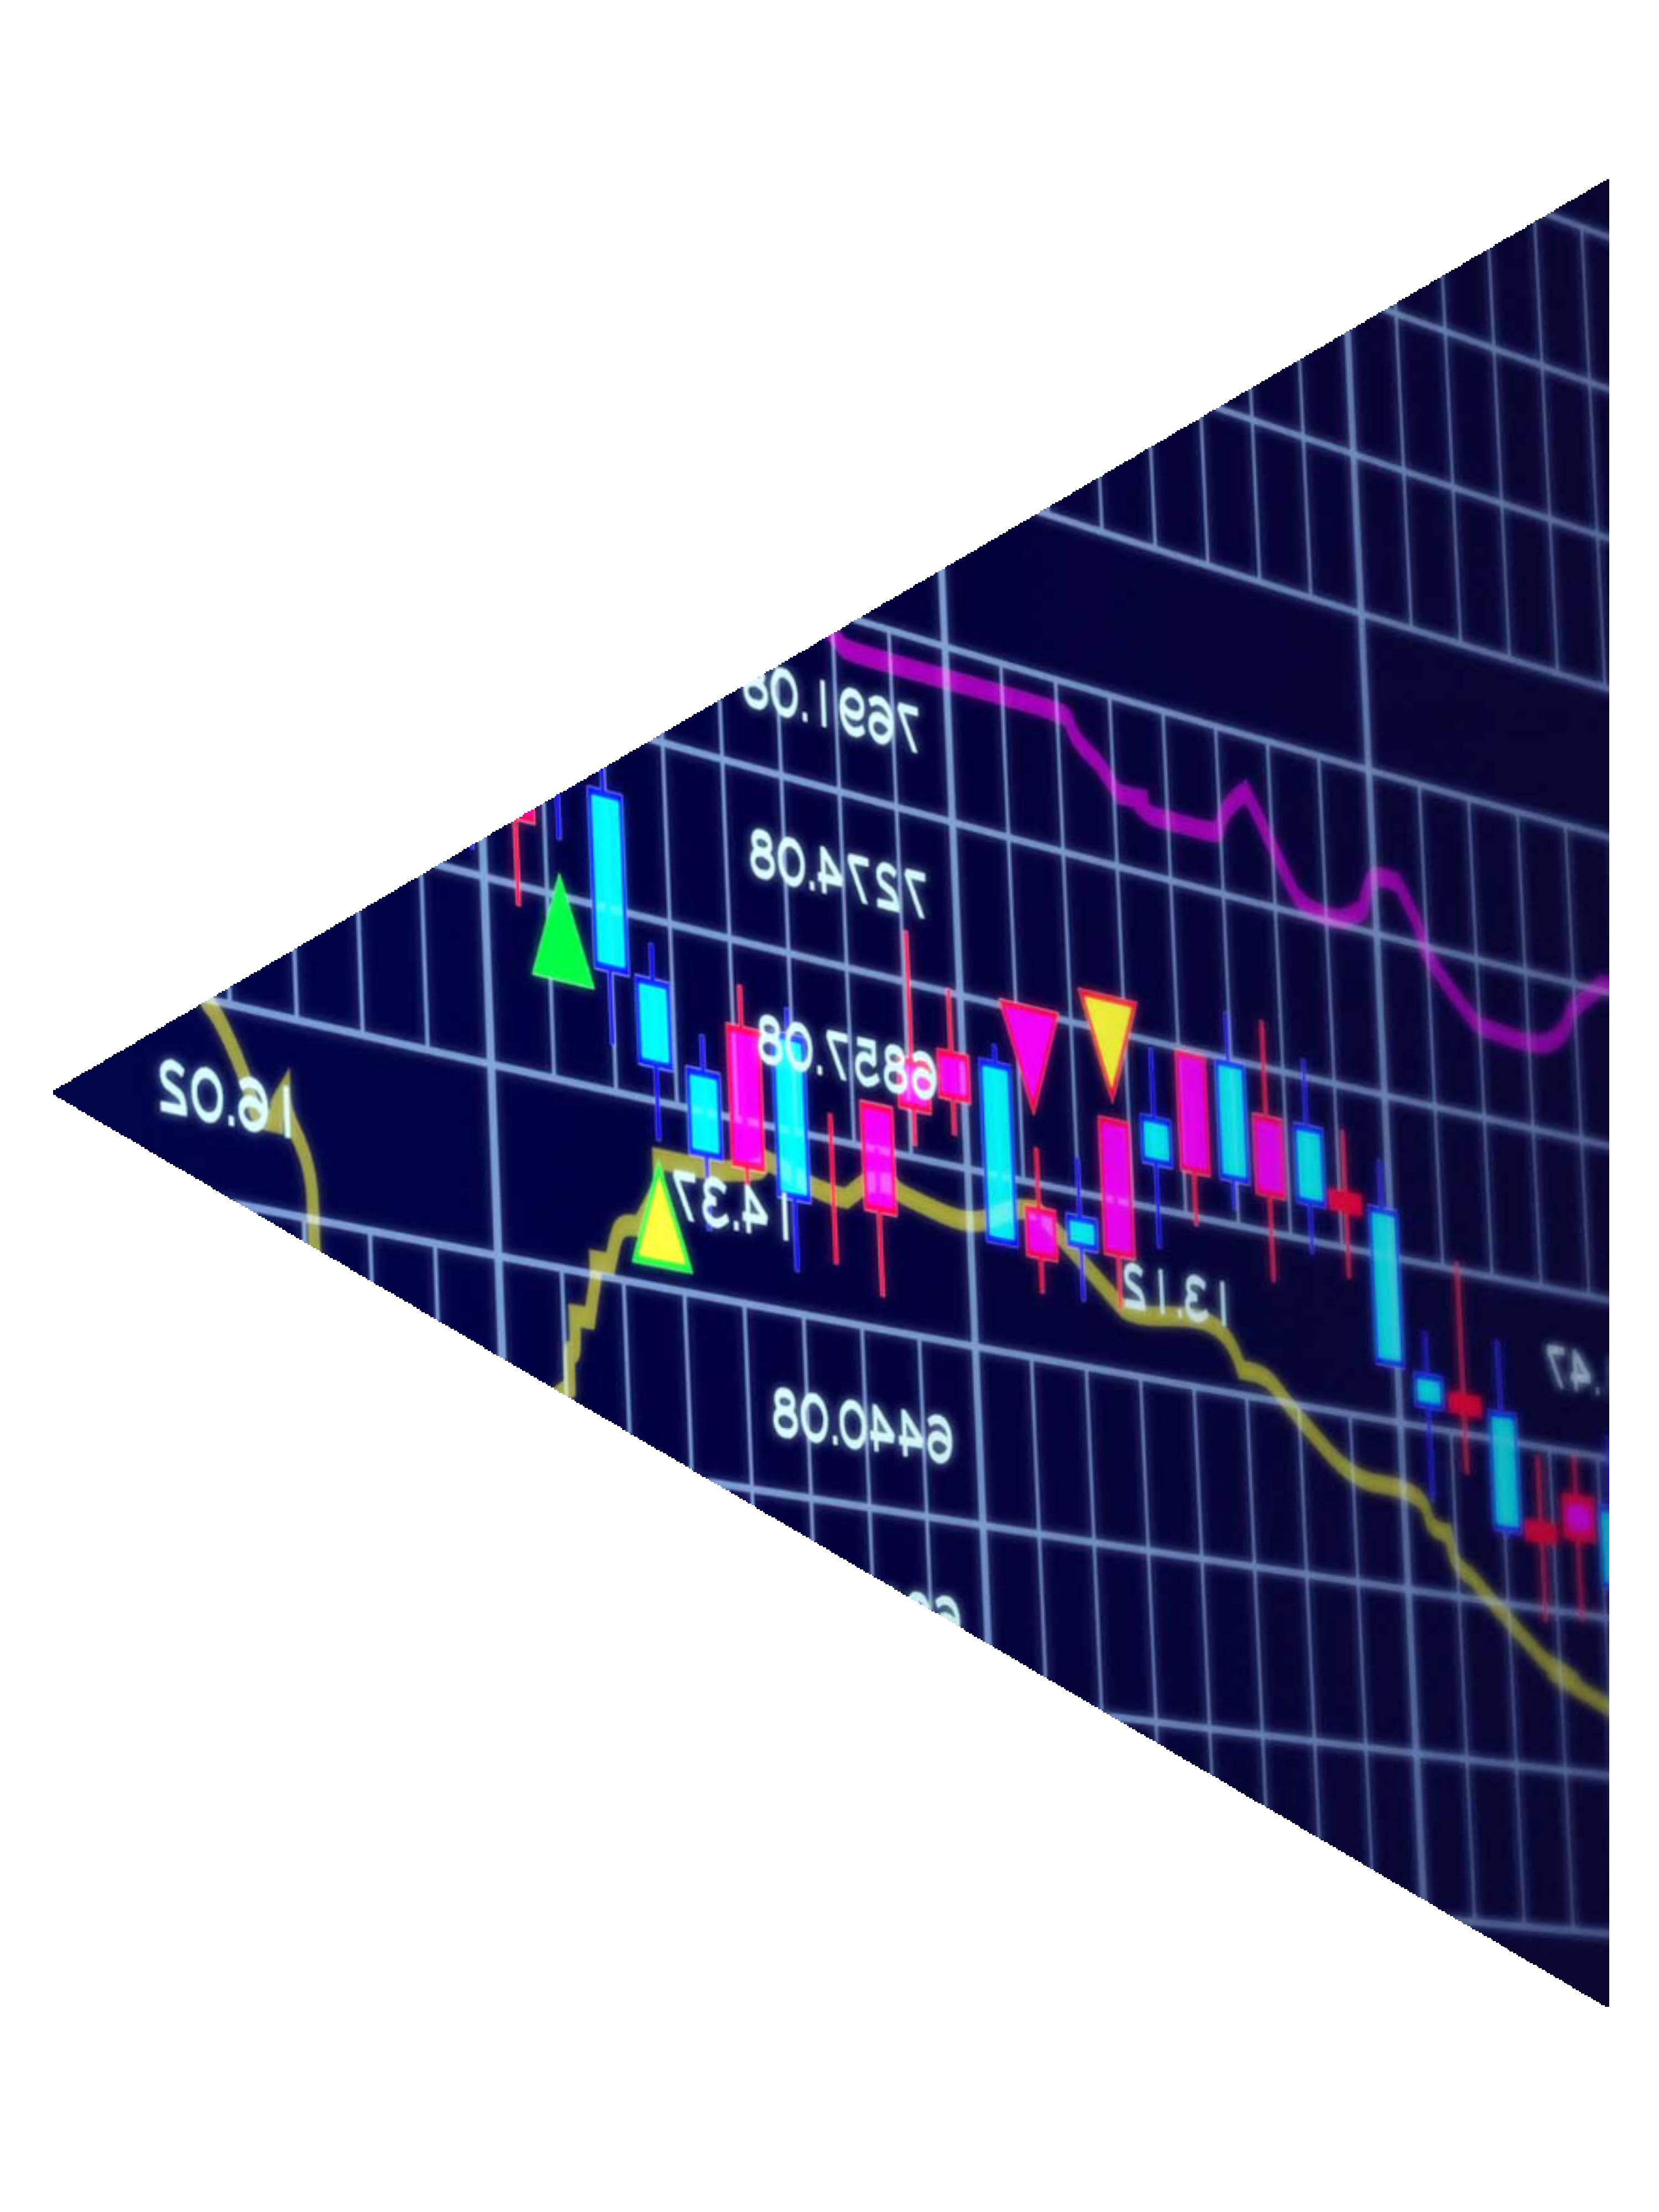
\includegraphics[width=22cm]{triangle.png}};
	\fill [jaune] (14,5) -- (2.5, 12) -- (20,25) -- (14, 20);
 \end{tikzpicture}}


\SetBgContents{\MyGraphicLogo}% Select included image

\SetBgPosition{current page.north west}% Select location
\SetBgOpacity{1.0}% Select opacity
\SetBgAngle{0.0}% Select roation of logo
\SetBgScale{1.0}% Select scale factor of logo



%%%%%%%%%%%%%%%%%%%%%%%%%%%%%%%%%%%%%%%%%%%%%%%%%%%%%%%%%%%%%%%%%%%%
%																																	   %
%																																	   %
%																																	   %
%										Informations générales sur le document															   %
%																																	   %
%																																	   %
%%%%%%%%%%%%%%%%%%%%%%%%%%%%%%%%%%%%%%%%%%%%%%%%%%%%%%%%%%%%%%%%%%%%

 \usepackage{fontspec}
  \usepackage[bold-style=upright]{unicode-math}
  \defaultfontfeatures{Scale=1}
  \setmainfont[Ligatures=TeX,Numbers=OldStyle]{Lucida Bright OT}
  \setmathfont[RawFeature=+ss04]{Lucida Bright Math OT}
  \setsansfont[Scale=1.0,Numbers=OldStyle]{Myriad Pro}
  \newfontfamily\fullcaps[Letters=Uppercase,Numbers=Uppercase]{Myriad Pro}
  \usepackage[babel=true]{microtype}
  \usepackage{icomma}
  
  \usepackage{amsmath,amsfonts,amssymb,amsthm,epsfig,epstopdf,titling,url,array}
  \theoremstyle{definition}
\newtheorem{defn}{Definition}[section]
  
  
  
  
  
  
  
  
  
\title{Implied volatility}
\author{Maxence COUPET - \href{mailto:maxence.coupet@gmail.com}{maxence.coupet@gmail.com}}
\date{March 2018}



\MHInternalSyntaxOn
\MH_set_boolean_T:n {outer_mult}
\MHInternalSyntaxOff

\newenvironment{nalign}{
    \begin{equation}
    \begin{aligned}
}{
    \end{aligned}
    \end{equation}
    \ignorespacesafterend
}
%%%%%%%%%%%%%%%%%%%%%%%%%%%%%%%%%%%%%%%%%%%%%%%%%%%%%%%%%%%%%%%%%%%%
%																																	   %
%																																	   %
%																																	   %
%												Mis en page du document																   %
%																																	   %
%																																	   %
%%%%%%%%%%%%%%%%%%%%%%%%%%%%%%%%%%%%%%%%%%%%%%%%%%%%%%%%%%%%%%%%%%%%


\begin{document}
	\selectlanguage{french}
	% page de garde
	\pagenumbering{gobble}
	\maketitle
	\newpage
	% début du rapport
	
	
	


\newcommand{\MyGraphicLog}{% For imported graphic logo
\begin{tikzpicture}[remember picture,overlay,yshift=-15cm, xshift=10.5cm]
\definecolor{jaune}{RGB}{16, 52, 78};
\fill[jaune] (-11, -16) -- (13, -16) -- (13, -12.1) -- (-11, -12.1);
 \end{tikzpicture}}


\SetBgContents{\MyGraphicLog}% Select included image


\SetBgPosition{current page.north west}% Select location
\SetBgOpacity{1.0}% Select opacity
\SetBgAngle{0.0}% Select roation of logo
\SetBgScale{1.0}% Select scale factor of logo

\pagestyle{fancy}
\renewcommand\headrulewidth{0pt}
\lhead{}\chead{}\rhead{}
\cfoot{\vspace*{6\baselineskip} \textcolor{white}{\thepage} \large}
	\newpage

	\pagenumbering{arabic}

%%%%%%%%%%%%%%%%%%%%%%%%%%%%%%%%%%%%%%%%%%%%%%%%%%%%%%%%%%%%%%%%%%%%
%																																	   %
%																																	   %
%																																	   %
%								Début du document (commencez à taper votre texte ici)													   %
%																																	   %
%																																	   %
%%%%%%%%%%%%%%%%%%%%%%%%%%%%%%%%%%%%%%%%%%%%%%%%%%%%%%%%%%%%%%%%%%%%

One must be aware of the differences between realized volatility and implied volatility. In most cases, when a market participant says ''volatility'' we must understand implied volatility.

\section{Realized volatility}

The realized volatility (or historical volatility) is the standard deviation of the logarithmic returns of an underlying. Let's consider $N$ historical prices for an underlying at different times $t_i$. The return will then be :
$$r_i = ln\left( \frac{S(t_i)}{S(t_{i-1})}\right)$$
Note that we could also have taken the return as the percentage change in each period. The mean of returns will be :
$$\bar{r}=\frac{1}{N} \sum_{i=1}^N r_i$$
and an unbiaised estimate of the standard deviation would be :
$$ \sigma = \sqrt{\frac{1}{N-1}\sum_{i=1}^N (r_i - \bar{r})^2}$$

A very important point with volatility is that it is always expressed as annualized volatility. So you will have to multiply this annualized volatility with the good time frame. For exemple, if we have a volatility $\sigma =20\%$ for a stock, the daily volatility is $\frac{\sigma}{\sqrt{252}} \approx 1.3 \%$. The value 252 represent the number of trading days in a year and is a common convention for the number of days in a year.

When we focus on realized volatility, we must keep in mind that the historical period has to be chosen very carefully since the historical data is not a good indicator of future performances in most cases.

\section{Implied volatility}

When using the historical volatility, we only have information about the past evolution of the underlying's volatility, we do not have any information about the current market sentiment and forecasting. This is what implied volatility intend to do. In order to compute implied volatility, we have to find very liquid derivatives, such as vanilla options. We then have a market price for the derivative, one price that all market participants agreed on. We can now use the Black-Scholes explicit formula, in order to find the volatility which would lead to the market price, this volatility is called the implied volatility. It is the market consensus on the futur value of the volatility. While they are often close, implied volatility and historical volatility are typically not equal. 

With this method, volatility is just an interpretation of the price of the derivative and most market participants will talk about buying certain amount of volatility instead of buying at a certain price, since it is the same information, but the value of volatility is more useful than the derivative's price for hedging considerations.

\section{Volatility skew}

As of now, we will not use explicit value for the strike of an option, but rather a percentage (ex : if the underlying price is 50\$ and the strike is 55\$, we will have a strike of 110\%). This notation is also very popular among market participants. 

One interesting property of the implied volatility, is something that the Black-Scholes model does not predict : the implied volatility has different values across strikes, as we can see in figure \ref{fig:skew}.

\begin{figure}[!h]
	\centering
	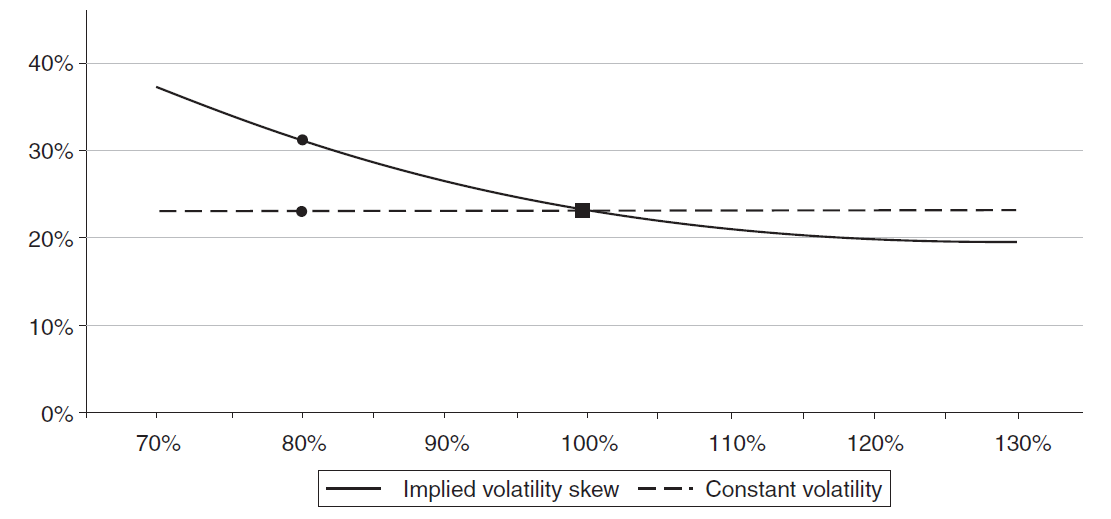
\includegraphics[width=\textwidth]{skew.png}
    \caption{Implied volatility and flat volatility across strikes}
    \label{fig:skew}
    \end{figure}
\end{document}